\documentclass[10pt]{article}
\usepackage{hyperref}
\usepackage{babel}
\usepackage{lastpage}
\usepackage{fancyhdr}
\usepackage[english]{babel}
\usepackage[vmargin=3cm]{geometry}
\usepackage{xcolor}
\usepackage[mmddyyyy]{datetime}
\usepackage{wrapfig}
\usepackage{minibox}
\usepackage[utf8x]{inputenc}
\usepackage{comment}
\usepackage{colortbl}
\usepackage{tabularx}
\usepackage{ocgx}
\usepackage{multirow}
\usepackage{lmodern}
\usepackage{tikz}
\usetikzlibrary{positioning}
\usepackage{float}
\usepackage[normalem]{ulem}
\usepackage{boldline}
\usepackage{framed}
\usepackage{bbding}
\usepackage{natbib}
\usepackage{url}
\usepackage{amsmath}
\usepackage{graphicx, xcolor, lipsum}
\usepackage{parskip}
\usepackage{pdfpages}
\usepackage{array}
\usepackage{amssymb}
\usepackage{gensymb}
\usepackage[colorlinks=true, linkcolor=black]{hyperref}
\usepackage{gbarcode}

% Creating a counter for the Property environment
%\newcounter{ctrProperty}
% Defining a custom Property environment
\newenvironment{openv}{%
   \refstepcounter{ctrProperty}%
   \textbf{\hspace{.2em}}\raggedright\itshape%
}{\par}



\newcommand{\n}{\newline}
\newcommand{\txt}{\textwidth}
\nonstopmode
\fancyhead[L]{

\includegraphics[scale= 0.2]{EMF_logo.jpg}
\hline
\textbf{Job:} 254249-1-1\\
\textbf{Customer} ALIANT TECH SYSTEMS OPEARATIONS LLC \\
\textbf{Customer PO} SP00125285 \\
\textbf{Container Type} Box
}
\fancyhead[C]{\colorbox{red}{\textbf{Job Traveler}} \\ 
\textbf{EXPEDITE} \\
\phantom{space} \\
\phantom{space} \\
\textbf{Containers:} 1 \textbf{Material:} 7075
}

\fancyhead[R]{Page \thepage\ of \pageref{LastPage} 
	\\
\textbf{Date:} \today \\
\textbf{Job Qty:} 2.00 \\
\textbf{Date Rec:} 8/18/2021 \\
CE
}
	
\headsep = 124pt 
\textheight = 500pt


\lfoot{EMF-400 Rev. A 9/3/2019}
\cfoot{}

\begin{document}
\pagestyle{fancy}
%part list start here
\begin{tabularx}{\txt}{p{12cm}p{3cm}}
	\hline
	%start repeat frame here
	\textbf{Part:} GW020K2013-1 & \textbf{Rev:} - \\
	\textbf{Description :} CONE, PANEL, ORD NO: 16GQ008769, REQ:
	PR-0450470\\
	\hline
	%end repeat frame here
	\end{tabularx}

%process list start here

\begin{tabularx}{\txt}{p{7cm}p{7.3cm}}
	\hline
\rowcolor{gray}\textbf{Process} & \textbf{Specification} \\
	\hline
	%start repeat frame here
	MASK  & AS NEEDED \\
	\hline
	%end repeat section here
	BR-127 Corrosion Inhibitor Primer & 597D1056 Rev.G BR-127 CORROSION INHIBITING PRIMER THICKNESS: 0.0002"-0.0006"\\
	\hline
	FINAL INSPECTION PAINT & 597D1056 REV.G PARA 7.3 \\
	\hline
\end{tabularx}
%Boolean galore
\begin{tabbing}
	\hspace{5cm} \= \hspace{5cm} \= \hspace{5cm} \kill
	\textbf{MASKING}? YES \> \textbf{BLUEPRINTS:} YES  \>  \textbf{FIRST ARTICLES?} YES \\ 
\end{tabbing}

\begin{framed}
	\colorbox{yellow}{Traveler Planning} \n
\begin{tikzpicture}{r}
	\pgfbarcode{13371337}
\end{tikzpicture}


\begin{wrapfigure}{r}{0.3\txt} 
\vspace{-\baselineskip}
\begin{tikzpicture}
\node(a)[label=
	above:{\scriptsize$PLANNER$}]{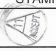
\includegraphics[width=1cm, height=1cm]{stamp1.png}};
\node(b)[right=1.5cm of (a), sep =10pts,
label=above:{\scriptsize$INSPECTOR$}]{
\includegraphics[width=1cm, height=1cm]{stamp2.png}};
\node(c)[draw, gray!40, minimum size=1.3cm, at=(a)]{};
\node(d)[draw, gray!60, minimum size=1.3cm, at=(b)]{};
\end{tikzpicture}

\end{wrapfigure}
\begin{openv}
\textbf{Additional Requirements} \\

Req. BY: 8/30/2021 %is this really necessary
\textbf{\textcolor{red}{Silicone Free Requirement}} \\

\scriptsize
ALL PROCESSES PERFORMED ARE SILICONE FREE BR-127, MATERIAL CERTS
ATTACHED 
BATCH# HG01LZ   EXP DATE:04-22

ADHESION TEST: PASS
\end{openv}
\end{framed}


% Now, in the same figure we draw two barcode: below is \texttt{ABC123} and above is \texttt{DEF456}:
% \begin{tikzpicture}
% \pgfbarcode{ABC123}

% \begin{pgfscope}
% \pgftransformshift{\pgfpoint{0}{10mm}}
% \pgfbarcode{DEF456}
% \end{pgfscope}
% \draw[blue,line width=1pt] (0,0)--(0,1);
% \end{tikzpicture}

%Another op code, if needed 
\begin{minipage}{\txt}
\begin{tabularx}{1.08\txt}{p{2cm}p{2cm}p{5cm}p{3cm}}
\textbf{Seq No}. & Oper. & Description & Oper. Qty \\
\hline 277 & INSPEC & FINAL INSPECTION-540 &2.00 \\
\end{tabularx}

\switchocg{ocg2}{\fcolorbox{green}{blue}{\bfseries +}}\begin{ocg}{OCG 2}{ocg2}{1}
\begin{tikzpicture}
\pgfbarcode{254248-1-277}
\end{tikzpicture}

\begin{framed}
\begin{wrapfigure}{r}{0.3\txt} 
\vspace{-\baselineskip}
\begin{tikzpicture}
\node(a)[label= above:{\scriptsize$PLANNER$}]{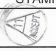
\includegraphics[width=1cm, height=1cm]{stamp1.png}};
\node(b)[right=0.75cm of (a), sep =10pts, label=above:{\scriptsize$DATE$}]{\framebox{\today \currenttime}};
\node(c)[draw, gray!60, minimum size=1.3cm, at=(a)]{};
%\node(d)[draw, gray!60, width =3cm, at=(b)]{};
\end{tikzpicture}
\end{wrapfigure}
\begin{openv}
	\scriptsize
FPL PASTE ETCH ref. \href{https://elitemetalfinishing.sharepoint.com/:b:/s/ComplianceGroup/EdoJDjFQVkNGoATbSYDrL8IBl5KBVNqIcdIP9ba9o7d2Ug?e=EEN44Q}{EMF-838}\n

1. APPLY FPL PASTE ETCH TO DESGINATED AREA AND ALLOW GEL TO REMAIN ON
SURFACE FOR 20-25 MINUTES  \n


ETCH TIME: \rule{2cm}{0.15mm}  \n

2. RINSE ALL ETCHED SURFACES WITH D.I. WATER FOR 10 MINUTES MIN.\n
3. OVEN DRY PARTS FOR  20 MINUTES MINIMUM \@ 120-150 \n
4. PRIMER MUST BE APPLIED WITHIN 8 HOURS OF THE ETCH STEP. \n


DATE COMPLETED: \rule{2cm}{0.15mm}\hspace{1cm} TIME
COMPLETED: \rule{2cm}{0.15mm}
\end{openv}
\end{framed}
\end{ocg}
\end{minipage}
%end opblock
\begin{minipage}{\txt}
\begin{tabularx}{1.08\txt}{p{2cm}p{2cm}p{5cm}p{3cm}}
\textbf{Seq No}. & Oper. & Description & Oper. Qty \\
\hline
277 & INSPEC & FINAL INSPECTION-540 &2.00 \\
\end{tabularx}

\switchocg{ocg1}{\fcolorbox{green}{blue}{\bfseries +}}\begin{ocg}{OCG 1}{ocg1}{0}
\begin{tikzpicture}
\pgfbarcode{254248-1-277}
\end{tikzpicture}

\begin{framed}
\begin{wrapfigure}{r}{0.3\txt} 
\vspace{-\baselineskip}
\begin{tikzpicture}
\node(a)[label=
	above:{\scriptsize$PLANNER$}]{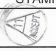
\includegraphics[width=1cm, height=1cm]{stamp1.png}};
\node(b)[right=0.75cm of (a), sep =10pts, label=above:{\scriptsize$DATE$}]{\framebox{\today \currenttime}};
\node(c)[draw, gray!60, minimum size=1.3cm, at=(a)]{};
%\node(d)[draw, green!60, minimum size=1.75cm, at=(b)]{};
\end{tikzpicture}
\end{wrapfigure}
\begin{openv}
	\scriptsize
FPL PASTE ETCH ref. EMF-838 (insert link here)\n

1. APPLY FPL PASTE ETCH TO DESGINATED AREA AND ALLOW GEL TO REMAIN ON
SURFACE FOR 20-25 MINUTES  \n


ETCH TIME: \rule{2cm}{0.15mm}  \n

2. RINSE ALL ETCHED SURFACES WITH D.I. WATER FOR 10 MINUTES MIN.\n
3. OVEN DRY PARTS FOR  20 MINUTES MINIMUM \@ 120-150 \n
4. PRIMER MUST BE APPLIED WITHIN 8 HOURS OF THE ETCH STEP. \n


DATE COMPLETED: \rule{2cm}{0.15mm}\hspace{1cm} TIME
COMPLETED: \rule{2cm}{0.15mm}
\end{openv}
\end{framed}
%end block
\end{ocg}
\end{minipage}

\begin{minipage}{\txt}
\begin{tabularx}{1.08\txt}{p{2cm}p{2cm}p{5cm}p{3cm}}
\textbf{Seq No}. & Oper. & Description & Oper. Qty \\
\hline
277 & INSPEC & FINAL INSPECTION-540 &2.00 \\
\end{tabularx}


\begin{tikzpicture}
\pgfbarcode{254248-1-277}
\end{tikzpicture}

\begin{framed}
\begin{wrapfigure}{r}{0.3\txt} 
\vspace{-\baselineskip}
\begin{tikzpicture}
\node(a)[label= above:{\scriptsize$PLANNER$}]{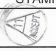
\includegraphics[width=1cm, height=1cm]{stamp1.png}};
\node(b)[right=0.75cm of (a), sep =10pts, label=above:{\scriptsize$DATE$}]{\framebox{\today \currenttime}};
\node(c)[draw, gray!60, minimum size=1.3cm, at=(a)]{};
%\node(d)[draw, green!60, minimum size=1.75cm, at=(b)]{};
\end{tikzpicture}
\end{wrapfigure}
\begin{openv}
	\scriptsize
FPL PASTE ETCH ref. EMF-838 (insert link here)\n

1. APPLY FPL PASTE ETCH TO DESGINATED AREA AND ALLOW GEL TO REMAIN ON
SURFACE FOR 20-25 MINUTES  \n


ETCH TIME: \rule{2cm}{0.15mm}  \n

2. RINSE ALL ETCHED SURFACES WITH D.I. WATER FOR 10 MINUTES MIN.\n
3. OVEN DRY PARTS FOR  20 MINUTES MINIMUM \@ 120-150 \n
4. PRIMER MUST BE APPLIED WITHIN 8 HOURS OF THE ETCH STEP. \n


DATE COMPLETED: \rule{2cm}{0.15mm}\hspace{1cm} TIME
COMPLETED: \rule{2cm}{0.15mm}
\end{openv}
\end{framed}
\end{minipage}

\end{document}
